\section{GeoSN Query Process System}

We overview the literature on GeoSN query processing systems in industry and academia. In what follows, we examine the API exposed by commercial online services, as well as the algorithm and data structure reported in academic projects.

\subsection{Commercial Products}
\subsubsection{Foursquare}
Foursquare’s Radar return the friends who are currently in the vicinity of a user. Foursqaure also expose their API for developers of LBS. The Foursquare API provides methods for accessing a resource such as a venue, tip, or user. In spirit with the RESTful model\cite{restful}, each resource is associated with a URL. For example, information about Clinton Street Baking Co can be found as follows (assuming credentials for such information is verified cryptographically beforehand):

\begin{verbatim}
	https://api.foursquare.com/v2/venues/40a55d80f964a52020f31ee3
\end{verbatim}

Given a resource, you can then drill into a particular aspect, for example

\begin{verbatim}
	https://api.foursquare.com/v2/venues/40a55d80f964a52020f31ee3/tips
\end{verbatim}

Each returned tip will have its own ID, which corresponds to its own resource URL, for example

\begin{verbatim}
	https://api.foursquare.com/v2/tips/49f083e770c603bbe81f8eb4
\end{verbatim}

Foursquare does not expose user's GPS location via its API, and only allows access to venue information (in the \texttt{venuehistory} and \texttt{checkins} aspects of user API). Foursquare also reveals the social network between users via the \texttt{friends} property of any users, which developers can use to get list of friends as follows:

\begin{verbatim}
	https://api.foursquare.com/v2/users/USER_ID/friends
\end{verbatim}

Foursquare does not report how they manage their social network database. However, they use MongoDB for the storage of venues and check-ins\cite{4qrmongo}. The original Foursquare application relied on a single relational database. With this relational architecture, foursquare could not simply and easily scale to many nodes required for a high traffic application. As the company experienced rapid growth, it split the data to two nodes: one for checkins (the biggest data set) and one for everything else. Yet it was clear that check-ins would grow beyond what a single machine could handle, and that a long-term, scalable solution to Foursquare's growth was needed. Foursquare benefits from MongoDB’s support for geospatial indexing, allowing it to easily query for location-based data. 

MongoDB's document model, with independent JSON-like objects, maps well to object-oriented programming, in contrast with the schema-enforced table structures of relational databases. MongoDB allows foursquare to dramatically simplify its data model. For instance, rather than storing tags ('has wifi", "great for dates", "hotspot", etc.) in a separate table and relying on mapping tables and costly JOINs, in MongoDB tags are embedded directly into the document representing a venue. This is both more efficient at run-time, and easier for engineers to understand and manipulate.

\subsubsection{Facebook}
Facebook's Graph API is the primary way for developers to get data in and out of Facebook's platform. Aside from social graph (stored using Memcached\cite{memcached}), developers can obtain user's location via \texttt{place} API as follows. 
Each place has a field called \texttt{overall\_rating}, which is the overall rating of Place, on a 5-star scale.

\begin{verbatim}
/* make the API call */
FB.api(
    "/{place-id}",
    function (response) {
      if (response && !response.error) {
        /* handle the result */
      }
    }
);
\end{verbatim}


Facebook's Local Awareness is an advertising solution designed to help local bricks-and-mortar and service businesses reach local customers efficiently. For instance, a local store promoting merchandise or sales can directly look for nearby homes and recent visitors; a local bank may choose to reach only people who live near their location; a local real estate agent may choose to reach only people who live near her properties for sale. 

Here is an ad set creation example (using cURL) that targets people who live or are visiting the area 10 miles around 1601 Willow Road Menlo Park CA, and excludes the zip code 94040:

\begin{verbatim}
curl \
  -F 'name=Local awareness adset' \
  ...
  -F 'targeting={ 
    "excluded_geo_locations": {"zips":[{"key":"US:94040"}]}, 
    "geo_locations": { 
      "custom_locations": [ 
        { 
          "latitude": 37.48327, 
          "longitude": -122.15033, 
          "radius": 10, 
          "distance_unit": "mile", 
          "address_string": "1601 Willow Road, Menlo Park, CA 94025" 
        } 
      ], 
      "location_types": ["home","recent"] 
    }, 
  }' 
\end{verbatim}

\subsubsection{ArcGIS}
ArcGIS\cite{arcgis} exposes a variety of functionalities to developers, including location services (directions/guidance, geo-trigger\footnote{Geo-trigger notifies a user when friends enter a certain range.}), mapping, and imagery. They claim that their data can be accessed via a RESTful API, but do not disclose details of how their data is managed. It is also unclear whether they have social networking functions in their system based on public information.

\subsection{Academic Efforts}
There has been few literature on GeoSN query processing\cite{amir2007buddy,yiu2010efficient,khoshgozaran2009private,scellato2010distance}. These works did not focus on important data management issues, which potentially undermine their practicality. More specifically, they tie the algorithms with specific data representations and indices, which may incurr significant overhead in large GeoSNs, because data representation scheme greatly affects the performance of any algorithm. Also, all of them assume that all the data are owned by a single entity, and can be handles by a single machine. More specifically:
\begin{itemize}
	\item\cite{khoshgozaran2009private,Liu} uses an adjacency matrix for keeping info about the social graph, which may incur prohibitive storage overhead;
	\item \cite{doytsher2012managing} uses adjacency lists stored in Neo4j\cite{developers2012neo4j};
	\item \cite{doytsher2010querying} utilizes relational tables for storing the friendship relations;
	\item\cite{amir2007buddy,scellato2010distance} make use of hybrid indices of both social and spatial data, which may suffer from enormous maintenance costs due to high check-in rates;
	\item\cite{yiu2010efficient,scellato2010distance} do not specify how the social graph is stored;
\end{itemize}

Academic research also has displayed a wide variety of indexing methods: \cite{amir2007buddy} applies a Quad tree, \cite{bao2012geofeed} indexes check-ins with a grid, and \cite{Liu} exploits the R*-Tree.

\subsection{A General Framework for Geo-Social Query Processing\cite{armenatzoglou2013general}}
A general framework for processing GeoSN queries is proposed in \cite{armenatzoglou2013general}.
The proposed architecture consists of three modules, depicted in Figure\ref{fig:gen-arch}: a social module (SM), a geographical module (GM), and a query processing module (QM). 
The SM stores only the social graph (e.g., friendship relations), and the GM keeps only geographical information (e.g., check-ins, venues, ratings). The QM is responsible for receiving GeoSN queries from users, executing them, and returning the results. The users do not communicate directly with the SM and GM. The SM, GM and QM can either be three separate servers, three separate clouds, or a single system (server or cloud). However, the tasks of the three modules are segregated.

\begin{figure}[hbt]
  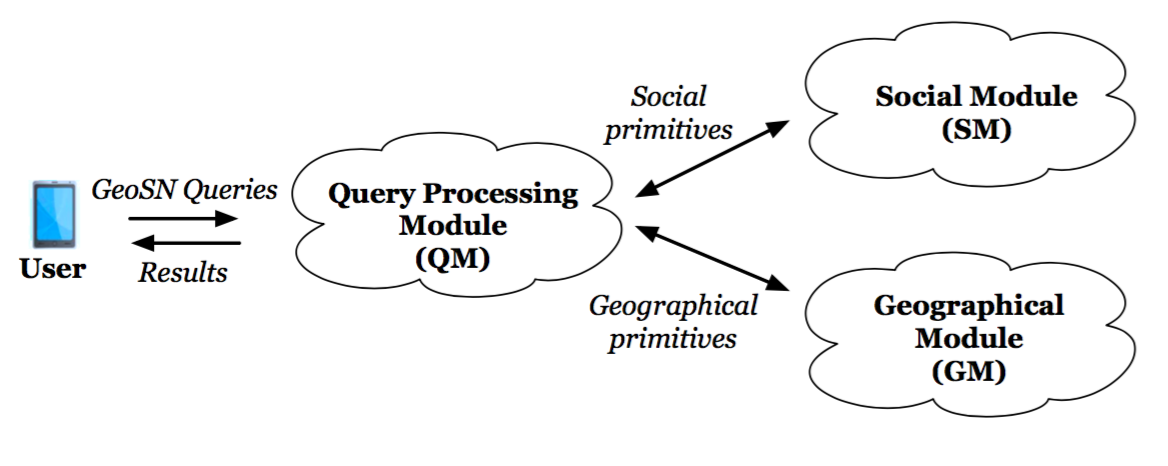
\includegraphics[width=\linewidth]{figs/gen-arch.png}
  \caption{The proposed architecture\cite{armenatzoglou2013general}}\label{fig:gen-arch}
\end{figure}

The SM and GM interact only with the QM using well-defined social and geographical primitive queries. 
The SM and GM only execute their corresponding primitives on their stored data, and the primitives are given by QM based on the algorithms used to process the queries. 
The QM eventually assembles the final results by combining the outputs of the primitives, optionally exploiting auxiliary indices maintained locally.

The segregation of SM and GM allows their administration by different entities, e.g., the SM (GM) can be maintained by a company with expertise in social networking (resp. location-based services)\cite{gen, factual}. For example, Facebook cooperates with Factual to provide infrastructure for location-based services. Cooperation of pure commercial social networks, e.g., Twitter or Facebook, and GeoSNs like Foursquare is also made possible by the separated architecture.. A user who has both a Twitter or Facebook and a Foursquare account can post his Foursquare check-in at Twitter or Facebook. Thus, if Facebook or Twitter needs the geographical information of users’ check-ins to execute a GeoSN query, it obtains it from Foursquare. The separation of QM enables third-party companies that do not own any social or geographical data to implement GeoSN queries by solely interacting with the APIs of SM and GM.

Separating the functionality of SM and GM renders the management of social and geographical data more flexible and more fault-tolerant, because the frequent check-in updates do not burden the relatively static social structures. 
For example, due to an unexpected high rate of check-ins recently, Foursquare’s system had a very long downtime. The problem was caused because their data are spread across multiple balanced database shards. When a shard is overused, a new one is added, followed by rebalancing. The rebalancing of the entire database caused the crash. In a segregated system, such a crash in GM would not affect SM.

This architecture can readily integrate modifications (e.g., a new, more efficient structure) in the implementation of SM without modifying GM, and vice versa. 

Another benefit is the extensibility in terms of adding novel GeoSN query types and algorithms. New queries can use a different combination of existing primitives. If the existing primitives are unable to implement the new queries/algortihms, new primitives can be added without the need of altering the SM and GM infrastructures\footnote{One caveat is that the new primitive must follow the design principle of separating SM and GM.}.

\subsection{Primitive Queries Proposed in \cite{armenatzoglou2013general}}
A set of primitives have been defined in \cite{armenatzoglou2013general} for the interfacing between SM/GM and QM. The social primitives are defined for SM-QM and geographical primitives are designed for GM-QM. These primitives arequeries that are building blocks in GeoSN algorithms. 

\textbf{Social primitives:}
\begin{itemize}
	\item GetFriends($u$): Given a user $u$, return $u$’s friends.
	\item AreFriends($u_i,u_j$): Given two users $u_i, u_j$, return $true$ if $u_i, u_j$ are friends, and $false$ otherwise.
\end{itemize}

\textbf{Geographical primitives:} 
\begin{itemize}
	\item GetUserLocation($u$): Given $u$, return $u$’s location.
	\item RangeUsers($q$, $r$): Given a query point $q$ and a real number $r$, return the users within distance $r$ from $q$, along with their locations.
	\item NearestUsers($q$,$k$): Given a query point $q$ and an integer $k$, return the $k$ users nearest to $q$ in ascending distance, along with their locations.
\end{itemize}

All the above primitives can be easily supported by the API of SM and GM. For example, GetFriends() is readily implemented in the API of Facebook Graph, and GetUserLocation() has the same functionality as the place field in Facebook's API. It is important to note that Facebook's API mixes social and geographical information, and implying the underlying design is not an implementation of the proposed architecture.

The efficiency of the primitives depends on the underlying storage scheme employed by SM and GM. For instance, representing the social graph by adjacency lists is preferable for GetFriends() (the output simply consists of the users in the list of $u$), whereas adjacency matrices are faster for AreFriends (the output is true if the bit at cell $(i,j)$ of the matrix is 1). Similarly, although all common spatial indices support RangeUsers and NearestUsers, they feature differences in performance.

\subsection{Summary}
We overview the API and architecture designs of GeoSN query processing systems. We examine the exposed API of online services, and investigate the academic literature on their assumptions of underlying data management methods for their algorithms. As noted in \cite{armenatzoglou2013general}, the best algorithm for each query type depends on the setting (data management method and system architecture). Finally, we focus on a general framework for query processing system. 

\begin{comment}
\end{comment}